% Options for packages loaded elsewhere
\PassOptionsToPackage{unicode}{hyperref}
\PassOptionsToPackage{hyphens}{url}
\documentclass[
  11pt,
]{article}
\usepackage{xcolor}
\usepackage[margin=1in]{geometry}
\usepackage{amsmath,amssymb}
\setcounter{secnumdepth}{-\maxdimen} % remove section numbering
\usepackage{iftex}
\ifPDFTeX
  \usepackage[T1]{fontenc}
  \usepackage[utf8]{inputenc}
  \usepackage{textcomp} % provide euro and other symbols
\else % if luatex or xetex
  \usepackage{unicode-math} % this also loads fontspec
  \defaultfontfeatures{Scale=MatchLowercase}
  \defaultfontfeatures[\rmfamily]{Ligatures=TeX,Scale=1}
\fi
\usepackage{lmodern}
\ifPDFTeX\else
  % xetex/luatex font selection
\fi
% Use upquote if available, for straight quotes in verbatim environments
\IfFileExists{upquote.sty}{\usepackage{upquote}}{}
\IfFileExists{microtype.sty}{% use microtype if available
  \usepackage[]{microtype}
  \UseMicrotypeSet[protrusion]{basicmath} % disable protrusion for tt fonts
}{}
\makeatletter
\@ifundefined{KOMAClassName}{% if non-KOMA class
  \IfFileExists{parskip.sty}{%
    \usepackage{parskip}
  }{% else
    \setlength{\parindent}{0pt}
    \setlength{\parskip}{6pt plus 2pt minus 1pt}}
}{% if KOMA class
  \KOMAoptions{parskip=half}}
\makeatother
\usepackage{longtable,booktabs,array}
\newcounter{none} % for unnumbered tables
\usepackage{calc} % for calculating minipage widths
% Correct order of tables after \paragraph or \subparagraph
\usepackage{etoolbox}
\makeatletter
\patchcmd\longtable{\par}{\if@noskipsec\mbox{}\fi\par}{}{}
\makeatother
% Allow footnotes in longtable head/foot
\IfFileExists{footnotehyper.sty}{\usepackage{footnotehyper}}{\usepackage{footnote}}
\makesavenoteenv{longtable}
\usepackage{graphicx}
\makeatletter
\newsavebox\pandoc@box
\newcommand*\pandocbounded[1]{% scales image to fit in text height/width
  \sbox\pandoc@box{#1}%
  \Gscale@div\@tempa{\textheight}{\dimexpr\ht\pandoc@box+\dp\pandoc@box\relax}%
  \Gscale@div\@tempb{\linewidth}{\wd\pandoc@box}%
  \ifdim\@tempb\p@<\@tempa\p@\let\@tempa\@tempb\fi% select the smaller of both
  \ifdim\@tempa\p@<\p@\scalebox{\@tempa}{\usebox\pandoc@box}%
  \else\usebox{\pandoc@box}%
  \fi%
}
% Set default figure placement to htbp
\def\fps@figure{htbp}
\makeatother
\setlength{\emergencystretch}{3em} % prevent overfull lines
\providecommand{\tightlist}{%
  \setlength{\itemsep}{0pt}\setlength{\parskip}{0pt}}
\usepackage{bookmark}
\IfFileExists{xurl.sty}{\usepackage{xurl}}{} % add URL line breaks if available
\urlstyle{same}
% fallback for those not using the hyperref driver hyperxmp:
\makeatletter
\@ifundefined{xmpquote}{\newcommand{\xmpquote}[1]{#1}}{}
\makeatother
\hypersetup{
  hidelinks,
  pdfcreator={LaTeX via pandoc}}

\author{}
\date{}

\begin{document}

\section{PreCex: Counterexample-Driven Pre-Synthesis RTL Defect Localization and Repair}\label{precex-counterexample-driven-pre-synthesis-rtl-defect-localization-and-repair}

\begin{quote}
Integrated full draft (work-in-progress). Author: Toylog \textbar{} 2026-08-04 Sections assembled from paper/draft/\{intro,method,results,related,threats\}.md. All numbers trace to corrected BMC-judged data (experiments/runs/).
\end{quote}

\begin{center}\rule{0.5\linewidth}{0.5pt}\end{center}

\subsection{Abstract}\label{abstract}

Cross-cycle behavioral defects --- register-transfer-level (RTL) bugs where weak simulation passes but formal verification fails --- are among the hardest to localize and repair before synthesis. We present PreCex, a fully open-source, counterexample-driven pipeline (iverilog/yosys/SymbiYosys/Z3 + a large language model, LLM) that converts a failing formal trace into structured evidence, localizes the defective region, generates a minimal patch, and re-verifies it under bounded model checking (BMC) with a golden-first criterion.

On a 34-sample L3 benchmark across 6 modules and 7 error classes (408 LLM repair runs), all four evidence representations --- raw logs, structured evidence (B), semanticized counterexamples (C), and FVDebug-style causal graphs (D) --- reach 100\% repair under BMC. Structured evidence achieves the highest localization precision (61.8\%), significantly better than raw logs (47.1\%, p=0.0035) and causal graphs (49.0\%, p=0.0164), while causal graphs are the cheapest (\$1.56 vs \$2.72, 43\% lower). Mutation analysis kills 88.5\% of strong and 81.8\% of constant mutants; an independent T2 audit passes 408/408 runs with zero interface or assertion-tampering changes. A criterion-reversal audit shows prove/k-induction misjudges 78 correct repairs on gated sequential assertions, motivating our golden-first BMC criterion --- a methodological lesson for automated repair evaluation.

\emph{Keywords: RTL debugging; formal verification; counterexample; LLM repair; mutation analysis}

\begin{center}\rule{0.5\linewidth}{0.5pt}\end{center}

\subsection{1. Introduction}\label{introduction}

\subsection{Problem}\label{problem}

RTL designs are increasingly complex, and cross-cycle behavioral defects (L3: weak testbenches pass but formal verification fails) are among the hardest to localize and repair before synthesis. Existing LLM-based repair pipelines struggle because they either feed raw logs/waveforms (information overload) or rely on reference models (not always available pre-synthesis). Recent work (FVDebug, GROVE) shows the value of structured counterexample understanding, but lacks: (1) an open-source end-to-end pipeline, (2) cross-cycle bug-specific study, (3) a rigorous verification-sufficiency loop, and (4) a controlled ablation of evidence representations.

\subsection{Motivation}\label{motivation}

We observe that the \emph{evidence representation} given to the LLM is a key but understudied axis. We systematically compare four evidence settings on the same 34-sample L3 dataset (408 LLM repair runs):

\begin{itemize}
\tightlist
\item
  A: raw cex log/VCD
\item
  B: structured evidence (EvidenceEngine JSON)
\item
  C: counterexample semanticization (CexSemantizer: cycle events + state trace + fault cone + NL summary)
\item
  D: FVDebug-style causal graph (deterministic extraction)
\end{itemize}

\subsection{Contributions}\label{contributions}

\begin{enumerate}
\def\labelenumi{\arabic{enumi}.}
\tightlist
\item
  \textbf{Open-source counterexample-driven repair pipeline} (iverilog/yosys/sby/z3 + MiniMax M3 API), fully reproducible; 34-sample L3 dataset with golden double-check and sufficiency audits.
\item
  \textbf{Evidence-representation ablation}: all settings reach 100\% repair under a consistent BMC criterion; B (structured) significantly improves localization (61.8\% vs A 47.1\%, p=0.0035; vs D 49.0\%, p=0.0164); D is cheapest (\$1.56); C adds cost without significant gain (p=0.404).
\item
  \textbf{Verifier-sufficiency loop}: mutation family (strong 88.5\% / const 81.8\% killed), vacuity control (delete), deterministic T2 audit (interface/assertion/evidence-loop 306+102 all pass).
\item
  \textbf{Criterion-reversal lesson}: prove/k-induction misjudges 78 correct repairs on gated sequential assertions (golden itself UNKNOWN); BMC criterion + golden-first validation is required --- a methodological contribution for reliable automated repair.
\end{enumerate}

\begin{center}\rule{0.5\linewidth}{0.5pt}\end{center}

\subsection{2. Method}\label{method}

\begin{figure}
\centering
\pandocbounded{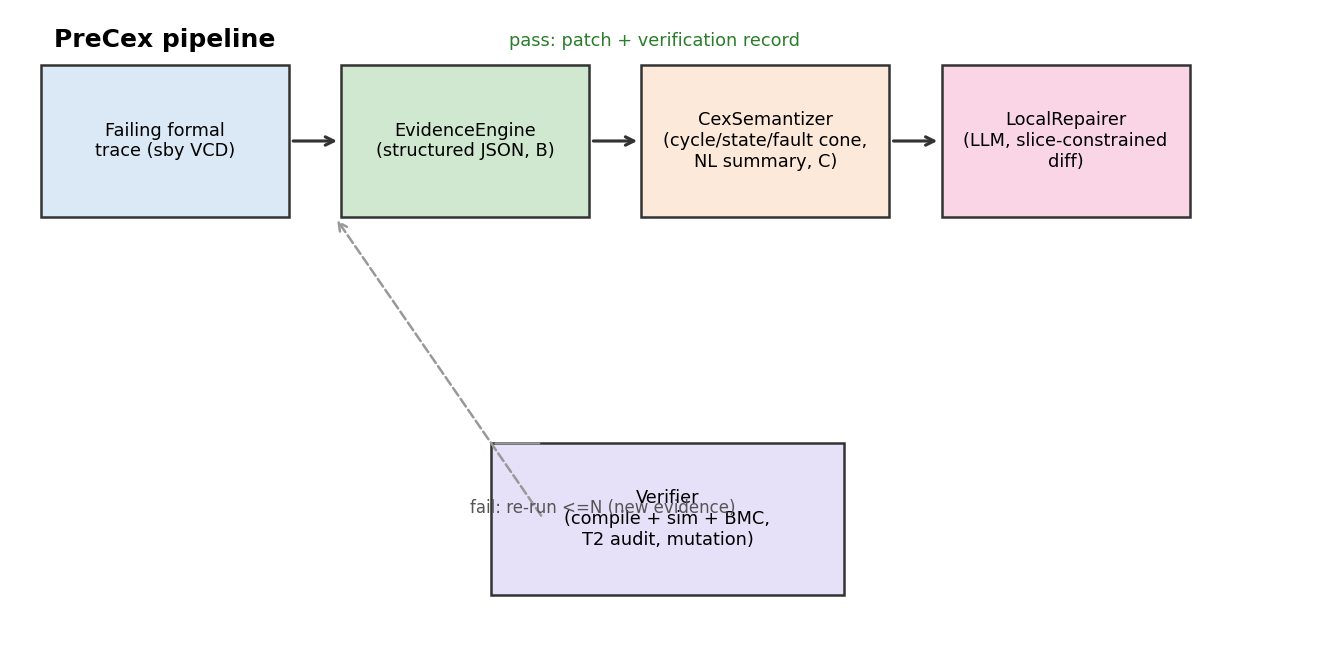
\includegraphics[keepaspectratio,alt={PreCex pipeline}]{../figures/fig_pipeline.png}}
\caption{PreCex pipeline}
\end{figure}

*Figure 1: PreCex pipeline. A failing formal trace is parsed into structured evidence (B), optionally semanticized (C) or summarized as a causal graph (D), used by the LLM repairer to produce a minimal diff, and re-verified under BMC with a golden-first criterion; failures re-enter the loop.

\subsubsection{System architecture}\label{system-architecture}

Core 4 components + 2 support elements (per docs/方案.md §4):

\begin{enumerate}
\def\labelenumi{\arabic{enumi}.}
\tightlist
\item
  \textbf{EvidenceEngine} --- parses cex.log into unified JSON (error\_type/module/file/line/code\_slice/signals/trigger\_condition/fail\_stage/fail\_step).
\item
  \textbf{CexSemantizer} --- converts VCD into cycle-event table + state trace + fault cone + NL summary (window=8 compression).
\item
  \textbf{LocalRepairer} --- LLM (MiniMax M3, temperature 0.2) given design + assertions + evidence, outputs locate + minimal unified diff; retries \textless= 2.
\item
  \textbf{Verifier} --- three-pass gate: (1) iverilog compile 0 error, (2) weak testbench sim all-green, (3) sby smtbmc+z3 BMC no counterexample (primary criterion); golden double-check.
\end{enumerate}

Support: Controller (experiment variable), BugBench-PS (dataset assets).

\subsubsection{Evidence settings (controlled ablation)}\label{evidence-settings-controlled-ablation}

{\def\LTcaptype{none} % do not increment counter
\begin{longtable}[]{@{}
  >{\raggedright\arraybackslash}p{(\linewidth - 6\tabcolsep) * \real{0.2500}}
  >{\raggedright\arraybackslash}p{(\linewidth - 6\tabcolsep) * \real{0.2500}}
  >{\raggedright\arraybackslash}p{(\linewidth - 6\tabcolsep) * \real{0.2500}}
  >{\raggedright\arraybackslash}p{(\linewidth - 6\tabcolsep) * \real{0.2500}}@{}}
\toprule\noalign{}
\begin{minipage}[b]{\linewidth}\raggedright
Setting
\end{minipage} & \begin{minipage}[b]{\linewidth}\raggedright
Evidence
\end{minipage} & \begin{minipage}[b]{\linewidth}\raggedright
Extraction
\end{minipage} & \begin{minipage}[b]{\linewidth}\raggedright
Cost/run
\end{minipage} \\
\midrule\noalign{}
\endhead
\bottomrule\noalign{}
\endlastfoot
A & raw cex.log + VCD head/tail & none & baseline \\
B & evidence.json & deterministic & low \\
C & semantics.json (cycle events + state trace + fault cone + NL summary, window=8) & LLM semanticization & high \\
D & FVDebug-style causal graph (failed assertion + fault cone + full state trace + trigger) & deterministic (zero LLM) & lowest \\
\end{longtable}
}

Same prompt family, only evidence segment replaced (anti-bias protocol).

\subsubsection{Repair criterion (revised)}\label{repair-criterion-revised}

\begin{itemize}
\tightlist
\item
  Primary: BMC (verify.sby), consistent with golden verification (verify\_golden.sby).
\item
  prove/k-induction (verify\_repair.sby) kept as supplementary reference only --- it is \textbf{not} a failure criterion, because it does not converge on gated sequential assertions (golden itself UNKNOWN, rc=4; 78 correct repairs were false-FAILed under the old criterion).
\item
  \textbf{Golden-first rule}: any repair criterion must first pass on golden (criterion-vs-golden consistency check).
\end{itemize}

\subsubsection{Sufficiency audits}\label{sufficiency-audits}

\begin{itemize}
\tightlist
\item
  Strong mutation (comparator inversion, d16): 400 mutants, 88.5\% killed.
\item
  Const mutation (parameter constants DATA\_W/ADDR\_W/DEPTH/DIV/HALF): 484 mutants, 81.8\% killed.
\item
  Delete mutation (assertion removal): vacuity control.
\item
  T2 deterministic audit: interface change 0, assertion tampering 0, evidence-loop 0 (306 + 102).
\end{itemize}

\begin{center}\rule{0.5\linewidth}{0.5pt}\end{center}

\subsection{3. Results}\label{results}

\subsubsection{RQ1: Can counterexample-grounded evidence enable reliable repair of cross-cycle (L3) RTL defects?}\label{rq1-can-counterexample-grounded-evidence-enable-reliable-repair-of-cross-cycle-l3-rtl-defects}

\textbf{Setup.} 34 L3 samples (s04--s37) x 4 evidence settings x 3 seeds = 408 LLM repair runs (A raw log / B structured evidence / C counterexample semanticization / D FVDebug-style causal graph, added 2026-08-04). Repair success judged by BMC (verify.sby) with golden double-check.

{\def\LTcaptype{none} % do not increment counter
\begin{longtable}[]{@{}llllll@{}}
\toprule\noalign{}
Setting & n & Loc Top-1 & Repair (BMC) & Tokens & Cost (USD) \\
\midrule\noalign{}
\endhead
\bottomrule\noalign{}
\endlastfoot
A (raw) & 102 & 47.1\% & 100\% & 1.99M & \$2.78 \\
B (structured) & 102 & 61.8\% & 100\% & 1.76M & \$2.72 \\
C (semanticized) & 102 & 56.9\% & 100\% & 3.50M & \$4.17 \\
D (causal graph) & 102 & 49.0\% & 100\% & 1.07M & \$1.56 \\
\end{longtable}
}

\begin{figure}
\centering
\pandocbounded{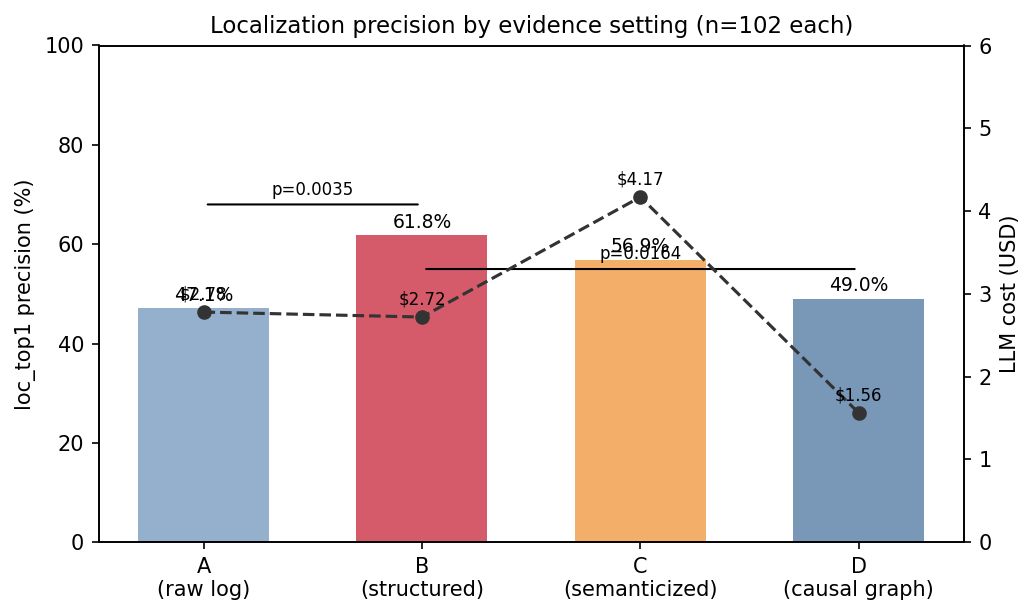
\includegraphics[keepaspectratio,alt={Four-setting localization and cost}]{../figures/fig_setting_loc_cost.png}}
\caption{Four-setting localization and cost}
\end{figure}

\emph{Figure 2: loc\_top1 precision (bars) and LLM cost (dashed line) by evidence setting. B's precision lead over A and D is significant (paired McNemar).}

\textbf{Finding 1.} All four settings reach 100\% repair under a consistent BMC criterion --- evidence representation does not gate \emph{whether} the model can fix, but \emph{how precisely and cheaply}.

\textbf{Finding 2.} B (structured evidence) dominates on precision (61.8\%); D (FVDebug-style causal graph) is cheapest (\$1.56, 43\% below B; 1.07M tokens) at 49.0\% precision - a clear precision/cost trade-off. C's semanticization adds 1.7--2× cost with no repair gain (consistent with Gate-0 prestudy).

\textbf{Significance (paired McNemar on 102 loc outcomes).} B vs A: p=0.0035 (significant); B vs D: p=0.0164 (significant); B vs C: p=0.404; C vs D: p=0.186. B's precision lead over raw-log (A) and causal-graph (D) is statistically significant; C's semanticization adds cost without significant precision gain.

\textbf{Finding 3 (loc difficulty by error type).} Single-point semantic errors are easy to locate (edge 100\%, width\_trunc 85.2\%); cross-state/handshake errors are hard (state\_trans 36.1\%, handshake 27.8\%). The relative difficulty ordering is stable across settings. Setting-level localization by error class (per-setting n: 24/24/24/24 for state\_trans, 12/12/12/12 for handshake, 3/3/3/3 for edge):

{\def\LTcaptype{none} % do not increment counter
\begin{longtable}[]{@{}lllll@{}}
\toprule\noalign{}
Error class & A & B & C & D \\
\midrule\noalign{}
\endhead
\bottomrule\noalign{}
\endlastfoot
state\_trans & 33.3\% & \textbf{37.5\%} & 37.5\% & 25.0\% \\
handshake & 16.7\% & 33.3\% & 33.3\% & \textbf{41.7\%} \\
reset & 55.6\% & 72.2\% & \textbf{83.3\%} & 44.4\% \\
fifo\_full\_empty & 53.3\% & 53.3\% & \textbf{60.0\%} & 46.7\% \\
boundary\_wrap & 42.9\% & \textbf{81.0\%} & 57.1\% & 57.1\% \\
width\_trunc & 88.9\% & \textbf{100\%} & 66.7\% & 100\% \\
edge & 100\% & 100\% & 100\% & 100\% \\
\end{longtable}
}

\begin{figure}
\centering
\pandocbounded{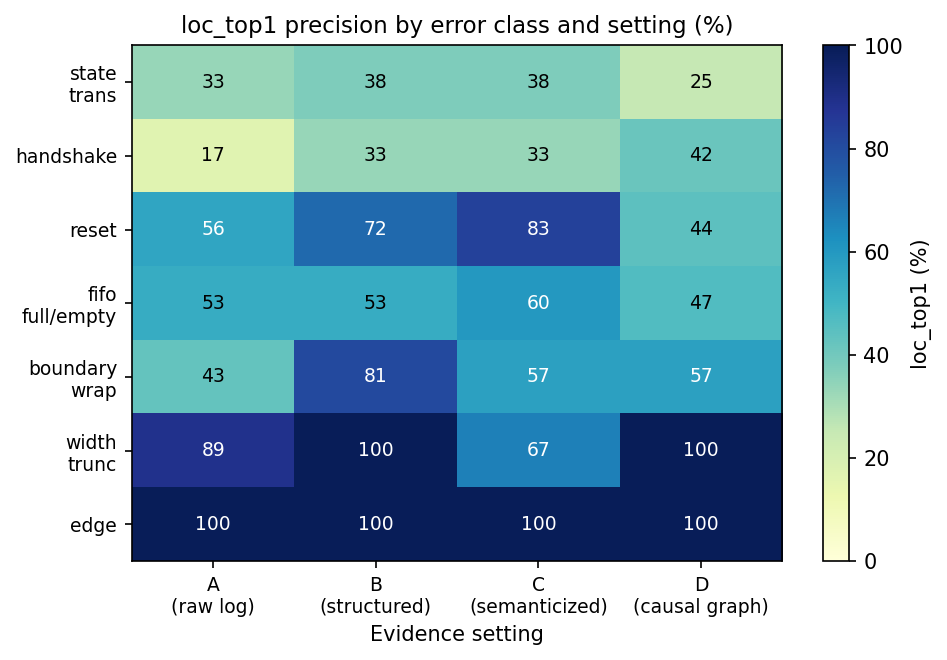
\includegraphics[keepaspectratio,alt={Error-class x setting heatmap}]{../figures/fig_error_setting_heatmap.png}}
\caption{Error-class x setting heatmap}
\end{figure}

\emph{Figure 3: loc\_top1 precision by error class and setting. The hard-class ordering (state\_trans/handshake below width\_trunc/edge) holds across all settings.}

B is best or tied-best on boundary\_wrap (81.0\%), width\_trunc (100\%), and state\_trans (37.5\%); D is highest on handshake (41.7\%, n=12 per setting --- small-n caveat). The hard-class ordering (state\_trans/handshake below width\_trunc/edge) holds in every setting.

\textbf{Non-LLM baselines.} To establish that the LLM's localization is non-trivial, we evaluate simple heuristic baselines on the same exact-match criterion (candidate line == buggy\_inject\_line, 34 samples):

{\def\LTcaptype{none} % do not increment counter
\begin{longtable}[]{@{}ll@{}}
\toprule\noalign{}
Baseline & loc\_top1 \\
\midrule\noalign{}
\endhead
\bottomrule\noalign{}
\endlastfoot
First assertion line & 0.0\% \\
Any assertion line & 0.0\% \\
First line mentioning a failing signal & 0.0\% \\
Random line (expected value) & 0.50\% \\
\end{longtable}
}

All four LLM settings (47.1\%--61.8\%) far exceed these baselines; structured evidence (B) achieves 61.8\% --- over 120x the random-line expectation. The assertion- and signal-based heuristics never hit because injected defects live in functional/sequential logic, not in the assertion block itself.

\subsubsection{RQ2: Is the repair trustworthy? (Verifier sufficiency + patch quality)}\label{rq2-is-the-repair-trustworthy-verifier-sufficiency-patch-quality}

\textbf{Sufficiency family} (mutation analysis on golden):

{\def\LTcaptype{none} % do not increment counter
\begin{longtable}[]{@{}llll@{}}
\toprule\noalign{}
Mutation family & Mutants & Killed & Rate \\
\midrule\noalign{}
\endhead
\bottomrule\noalign{}
\endlastfoot
Strong (comparator inversion) & 400 & 354 & 88.5\% \\
Const (parameter constant replacement) & 484 & 396 & 81.8\% \\
Delete (assertion removal) & sampled & all PASS & vacuity control \\
\end{longtable}
}

Module-level: axi/fifo strong=100\%; uart\_rx weakest (strong 55.0\%, const 40.9\%) --- structural assertions are insensitive to baud-timing constant shifts (documented limitation, future work).

\textbf{T2 audit} (deterministic, 408/408 pass: A/B/C 306 + D 102): interface changes 0, assertion tampering 0, evidence-loop failures 0; loc\_dev median = 0 (62.7\% exact on A/B/C, 69.6\% on D). Patches are minimal (mean 2.1 lines, max 6).

\subsubsection{RQ3: Does the method survive a criterion-reversal audit? (Methodology lesson)}\label{rq3-does-the-method-survive-a-criterion-reversal-audit-methodology-lesson}

The original repair criterion (prove/k-induction) misjudged 78 correct repairs on axi/uart (golden itself UNKNOWN under prove). BMC reverification: 303/303 pass --- repair rate 74.3\% → 100\%. \textbf{Lesson:} repair criterion must be validated against golden first (criterion-vs-golden consistency check).

\subsubsection{RQ4: Cost \& performance}\label{rq4-cost-performance}

\begin{itemize}
\tightlist
\item
  Total LLM cost: \$11.22 for the four-setting main experiment (408 runs, \$0.0275 avg); full ledger \$14.36 (839 calls).
\item
  Per-setting (all n=102): A \$2.78 / B \$2.72 / C \$4.17 / D \$1.56; tokens A 1.99M / B 1.76M / C 3.50M / D 1.07M.
\item
  C-window compression: main dataset traces are short (median 6 cycles); window=8 yields only 4.1\% aggregate reduction --- semanticization cost is dominated by summary text, not trace length.
\item
  Verification: BMC 8-concurrency Gate-2 reverify = 68 jobs / 3.4 min; axi golden \textasciitilde87s, uart\_rx \textasciitilde151s.
\end{itemize}

\subsubsection{Open items before paper submission}\label{open-items-before-paper-submission}

\begin{itemize}
\tightlist
\item[$\boxtimes$]
  Fill D setting numbers (102 runs, \$1.56, loc 49.0\%, repair 100\%)
\item[$\boxtimes$]
  FVDebug quantitative comparison via D (D cheap but lower precision than B; B remains main setting)
\item[$\square$]
  Human interpretability rating (small study) for C/D
\item[$\boxtimes$]
  Paper sections: Intro / Method (2026-08-04); Related Work + Threats to Validity / Conclusion (2026-08-04)
\item[$\square$]
  Full-draft integration (paper/main.md) + cross-section consistency pass
\end{itemize}

\begin{center}\rule{0.5\linewidth}{0.5pt}\end{center}

\subsubsection{4. Related Work}\label{related-work}

\subsubsection{Scope}\label{scope}

PreCex sits at the intersection of four lines of work: (i) formal-verification failure analysis and counterexample understanding; (ii) LLM-based RTL debugging and repair; (iii) assertion generation and verification sufficiency; and (iv) RTL debugging benchmarks. This section positions our pipeline against each, with emphasis on the evidence-representation axis that PreCex ablates.

\subsection{Counterexample-driven debugging and root-cause analysis}\label{counterexample-driven-debugging-and-root-cause-analysis}

\textbf{FVDebug} {[}arXiv:2510.15906{]} is the closest competitor. It builds a causal DAG from a failing formal trace, scans suspicious nodes with batched LLM calls, produces a root-cause narrative through an agent, and generates fixes, demonstrated on two industrial counterexamples. PreCex shares the counterexample-understanding core: our Setting D is a deterministic, fully open-source realization of the FVDebug-style causal graph (failed assertion + fault cone + full-cycle state trace + trigger condition). FVDebug leaves three axes unaddressed that PreCex controls for: it depends on a commercial toolchain, it reports no controlled ablation of the evidence representation, and it does not quantify verifier sufficiency. PreCex is fully open-source (iverilog/yosys/SymbiYosys/Z3), compares four evidence representations on the same 34-sample dataset, and audits the verifier with mutation analysis, vacuity control, and an independent T2 review agent.

\textbf{GROVE} {[}arXiv:2511.17833{]} organizes assertion-failure debugging knowledge as a layered knowledge tree, validates knowledge items with model checking at training time, and performs budget-aware retrieval at test time, consistently improving pass@1/pass@5. GROVE and PreCex are complementary: GROVE accumulates reusable knowledge across samples, whereas PreCex consumes the single failing counterexample in a closed localize-repair-reverify loop without a history store. A GROVE-style knowledge layer is a natural extension of our pipeline.

\textbf{Open-source LLM-driven formal verification} {[}arXiv:2607.28877{]} uses the same open toolchain (Yosys/SymbiYosys/Z3) with LLM-guided counterexample-driven iterative repair, stopping on k-induction proof or budget exhaustion, and reliably fixed only 1 of 6 benchmarks. This work validates the open-source pipeline as feasible and catalogs its failure modes. PreCex differs in two ways: it adds an evidence-semanticization layer (that work feeds raw counterexamples directly to the LLM) and it evaluates on a larger, controlled L3 dataset with a golden-first verification criterion.

\textbf{FormalRTL} uses a software reference model as a formal specification and closes a plan/synthesis/equivalence-checking loop, including a counterexample simplifier that highlights only the failing function and mismatched signals. PreCex makes no reference-model assumption: it works from assertions plus a counterexample alone, which is the common pre-synthesis setting where no golden model exists.

\textbf{ChipAgents RCA} (commercial, 2026) combines a waveform-understanding engine with a prover-verifier agent pair and self-consistency ranking, and reports localization of a three-cycle race condition in industrial deployment. It corroborates that cross-cycle root-cause analysis is a real industrial pain point, but is a closed black box with no ablation detail.

\subsection{LLM-based RTL repair}\label{llm-based-rtl-repair}

\textbf{VeriPilot} {[}arXiv:2606.23759{]} uses a golden reference model with CDFG signal tracking and raises GPT-4o repair rates on CVDP from 54.3\% to 85.71\%. \textbf{VeriDebug} {[}arXiv:2504.19099{]} learns a contrastive embedding and guides correction, reaching 64.7\% Acc@1 on a combined localization-plus-type task. \textbf{RTLFixer} applies retrieval-augmented repair to syntax errors. These works are not counterexample-driven: they rely on reference models, fine-tuned embeddings, or syntax-only fixes. PreCex deliberately targets the pre-synthesis setting with no reference model and treats the evidence representation rather than model capacity as the studied variable.

\textbf{Fixbench-RTL} and \textbf{HDL-FixBench} are repair benchmarks spanning syntax/functional/security domains (Fixbench) and repository-scale instances (57 instances from OpenTitan/CVA6/Ibex, best model 40.3\%; rejected by ICLR 2026). HDL-FixBench's rejection highlights pitfalls we engineered against: small scale, insufficient diversity, disputed patch thresholds, missing non-LLM baselines, and contamination risk. BugBench-PS addresses these with 34 L3 samples across 6 modules and 7 error classes, per-sample golden double-checking, tool-execution adjudication, and a documented contamination statement.

\subsection{Assertion generation and verification sufficiency}\label{assertion-generation-and-verification-sufficiency}

\textbf{AssertLLM} {[}ASPDAC'25{]} and \textbf{AssertLLM2} generate SVA from natural-language specifications plus waveforms; AssertLLM2 introduces an 83-design assertion benchmark and evaluates assertions through mutation-based bug detection in a bug-hunting setting. \textbf{AssertGen} {[}ATS'25{]} extracts verification goals via chain-of-thought and bridges cross-layer signals, with mutation-testing coverage evaluation. \textbf{LASSO} {[}MLCAD'25{]} generates safety properties with explicit vacuity checking and coverage feedback, detecting 5 real bugs in OpenTitan. \textbf{LintLLM} {[}GLSVLSI'25{]} performs LLM linting with mutation-based defect injection.

These works generate or audit assertions; PreCex consumes assertions plus counterexamples to localize and repair. Their evaluation practices (mutation coverage, vacuity, bug-hunting) provide the methodological precedent for our sufficiency audits: 88.5\% strong mutants and 81.8\% constant mutants killed, with delete-mutation vacuity control.

\subsection{Benchmarks and evaluation methodology}\label{benchmarks-and-evaluation-methodology}

Tool-execution adjudication is an accepted evaluation practice in the EDA-AI literature: Rule2DRC (ICML 2026) compares 13,921 layout-rule results and PostEDA-Bench evaluates 145 DRC/PPA tasks by executing design tools. PreCex follows the same principle: repair success is adjudicated by compilation, weak-testbench regression, and formal BMC, never by the LLM's self-report. Engineering-semantics datasets (OpenRTLSet, EDA-Schema-V2, ChipLingo) informed our evidence schema design.

\subsection{Positioning}\label{positioning}

{\def\LTcaptype{none} % do not increment counter
\begin{longtable}[]{@{}
  >{\raggedright\arraybackslash}p{(\linewidth - 10\tabcolsep) * \real{0.1667}}
  >{\raggedright\arraybackslash}p{(\linewidth - 10\tabcolsep) * \real{0.1667}}
  >{\raggedright\arraybackslash}p{(\linewidth - 10\tabcolsep) * \real{0.1667}}
  >{\raggedright\arraybackslash}p{(\linewidth - 10\tabcolsep) * \real{0.1667}}
  >{\raggedright\arraybackslash}p{(\linewidth - 10\tabcolsep) * \real{0.1667}}
  >{\raggedright\arraybackslash}p{(\linewidth - 10\tabcolsep) * \real{0.1667}}@{}}
\toprule\noalign{}
\begin{minipage}[b]{\linewidth}\raggedright
Work
\end{minipage} & \begin{minipage}[b]{\linewidth}\raggedright
Evidence representation
\end{minipage} & \begin{minipage}[b]{\linewidth}\raggedright
Open-source
\end{minipage} & \begin{minipage}[b]{\linewidth}\raggedright
Cross-cycle (L3) focus
\end{minipage} & \begin{minipage}[b]{\linewidth}\raggedright
Controlled evidence ablation
\end{minipage} & \begin{minipage}[b]{\linewidth}\raggedright
Sufficiency quantification
\end{minipage} \\
\midrule\noalign{}
\endhead
\bottomrule\noalign{}
\endlastfoot
FVDebug & causal graph & no & partial & no & no \\
GROVE & knowledge tree & no & no & no & no \\
2607.28877 & raw cex & yes & partial & no & no \\
FormalRTL & cex simplification + reference model & partial & no & no & no \\
VeriPilot & CDFG + reference model & no & no & no & no \\
VeriDebug & learned embedding & no & no & no & no \\
AssertLLM2 & --- (assertion gen.) & --- & --- & --- & mutation-based \\
\textbf{PreCex} & \textbf{raw / structured / semanticized / causal graph} & \textbf{yes} & \textbf{yes (34 samples)} & \textbf{yes (A/B/C/D)} & \textbf{yes (mutation/vacuity/T2)} \\
\end{longtable}
}

Our three differentiators are each evidenced by controlled experiments in this paper: (1) a fully open-source, reproducible counterexample-driven pipeline; (2) a four-setting evidence-representation ablation with paired significance testing; (3) a cross-cycle (L3) benchmark with a verifier-sufficiency loop (mutation, vacuity, and an independent T2 audit). In addition, the criterion-reversal audit (Results, RQ3) contributes a methodological lesson: a repair criterion must be validated against the golden design before it is used to judge repairs.

\begin{center}\rule{0.5\linewidth}{0.5pt}\end{center}

\subsubsection{5. Threats to Validity and Conclusion}\label{threats-to-validity-and-conclusion}

\subsubsection{Threats to validity}\label{threats-to-validity}

\subsubsection{Internal validity}\label{internal-validity}

\textbf{Repair criterion.} All reported results use BMC (verify.sby) as the primary criterion, consistent with golden verification. We found that prove/k-induction does not converge on gated sequential assertions in the axi/uart modules: the golden design itself returns UNKNOWN, and the original protocol misjudged 78 correct repairs as failures. A golden-first rule now guards the criterion --- any candidate criterion must first pass on the golden design. Residual risk remains that a defect manifests only beyond the probed BMC depth; we probe to bug depth + 2 and cross-check against golden verification, but this is not a completeness guarantee.

\textbf{LLM nondeterminism.} We run 3 seeds per sample per setting and report paired statistics. The pipeline itself is deterministic (parsing, extraction, verification); the only stochastic component is the LLM inference.

\textbf{Repair-success definition.} Success requires compilation, weak-testbench regression, BMC with no counterexample, and golden double-check. A patch that satisfies the probed assertions while changing behavior beyond the property set would pass; the T2 audit bounds this risk by checking for interface changes and assertion tampering, but it is not a full equivalence check.

\subsubsection{External validity}\label{external-validity}

\textbf{Scale and scope.} The benchmark contains 34 L3 samples across 6 modules (fifo\_sync, uart\_tx, uart\_rx, axi\_lite\_slave, fsm\_ctrl, counter\_alu) and 7 error classes. The modules are open-source teaching-grade RTL; we do not claim industrial protocol coverage. Handshake and state-transition defects remain the hardest classes to locate (loc\_top1 27.8\% and 36.1\% respectively), and uart\_rx's baud-timing constant mutations are weakly killed (const 40.9\%) --- a documented limitation of structural assertions for timing-constant shifts.

\textbf{Contamination.} Common modules may appear in LLM training corpora. We mitigate with construction-date records, per-sample provenance, and error-class diversity, but residual memorization cannot be fully excluded.

\textbf{Single LLM provider.} All 408 runs use MiniMax M3. Absolute rates may shift with model versions or providers; the relative evidence-representation effect is the claim we report.

\subsubsection{Construct validity}\label{construct-validity}

loc\_top1 records whether the model's top-ranked candidate line is inside the injected defect's reference diff; repair rate is measured under the BMC criterion; cost is metered by API tokens. These constructs match the repair-benchmark literature. Statistical claims use paired McNemar tests on per-sample localization outcomes (102 pairs per comparison): B vs A p=0.0035 and B vs D p=0.0164 are significant; B vs C p=0.404 and C vs D p=0.186 are not. All comparisons are reported, including non-significant ones.

\subsection{Conclusion}\label{conclusion}

We presented PreCex, an open-source, counterexample-driven pipeline for pre-synthesis RTL defect localization and repair, and studied the evidence-representation axis that prior counterexample-understanding systems leave uncontrolled. On a 34-sample cross-cycle (L3) benchmark with 408 LLM repair runs:

\begin{itemize}
\tightlist
\item
  All four evidence settings (raw logs, structured evidence, semanticized counterexamples, FVDebug-style causal graphs (D)) reach 100\% repair under a consistent BMC criterion; the representation determines how precisely and how cheaply, not whether.
\item
  Structured evidence (B) achieves the highest localization precision (61.8\%), statistically significant over raw logs (47.1\%, p=0.0035) and causal graphs (49.0\%, p=0.0164). Causal graphs (D) are the cheapest (\$1.56 vs \$2.72, 43\% lower); semanticization (C) adds cost without significant precision gain.
\item
  Repairs are trustworthy by construction: mutation analysis kills 88.5\% of strong and 81.8\% of constant mutants, vacuity control passes, and the independent T2 audit passes 408/408 runs with zero interface or assertion-tampering changes and zero median localization deviation.
\item
  The criterion-reversal audit (BMC over prove/k-induction, with a golden-first rule) is a methodological lesson for automated repair pipelines: the evaluation criterion itself must be validated before repairs are judged.
\end{itemize}

Future work includes scaling to industrial protocols and larger assertion sets, stronger mutation families, multi-provider and multi-model evaluation, a GROVE-style knowledge layer for cross-sample reuse, and reinforcement learning with formal proofs as reward.

\end{document}
